\newpage
\section{Critical Design}
\label{sec:critical_design}

The basic \ac{EPS} diagram is shown in  Figure \ref{fig:EPS_diagram_simple}. A \ac{SAR} controls the operating voltage of the solar array and supplies an unregulated mainbus. The mainbus voltage is mainly controlled by the battery voltage. A DC-DC regulator provides a regulated $5\,V$ supply to subsystems and payloads. Motors are supplied from the unregulated mainbus.

\begin{figure}[H]
\centering
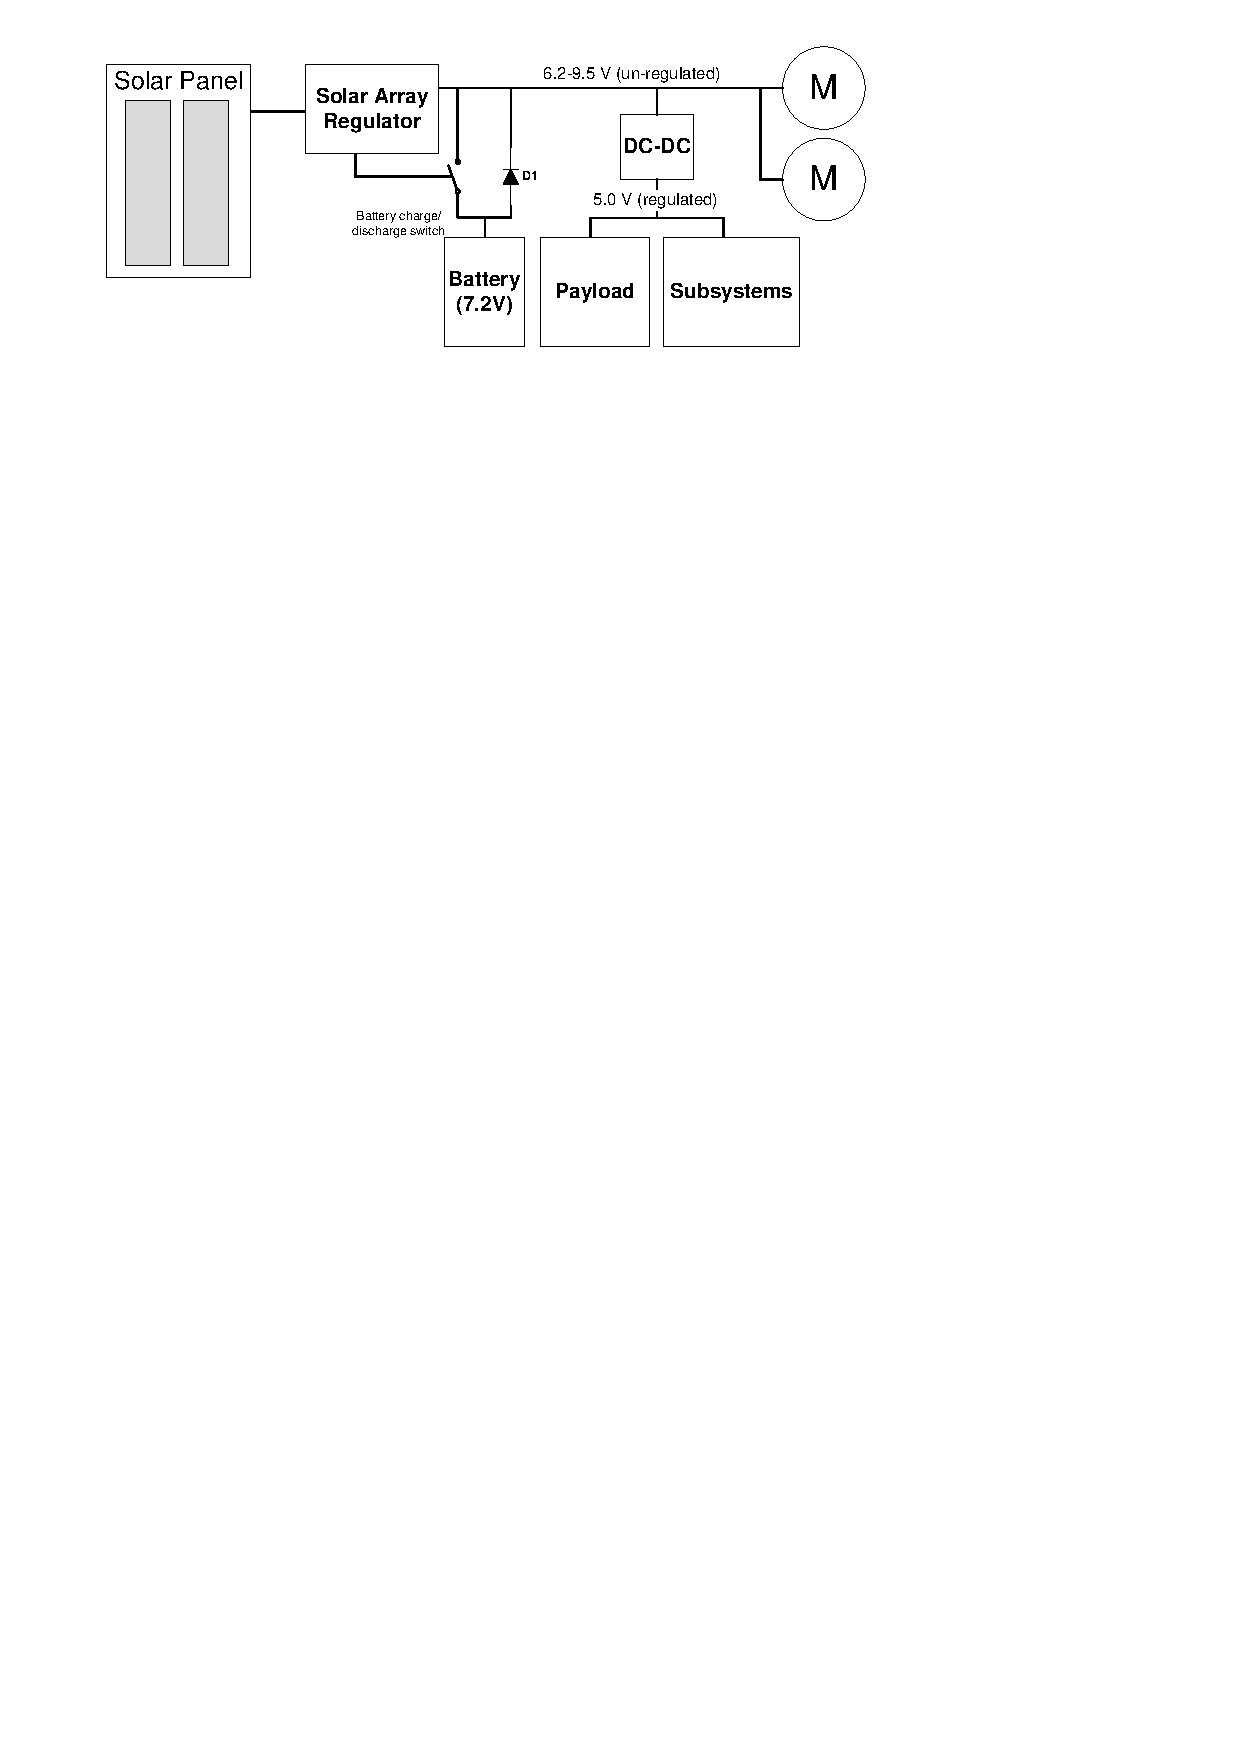
\includegraphics[width=\textwidth]{figures/fig_PDR_EPSdiagram}
\caption{\ac{EPS} simple blockdiagram}
\label{fig:EPS_diagram_simple}
\end{figure}
%
%
\subsection{Solar Array Design}
The \textit{PowerFilm RC7.2-75(PSA)} solar cell is selected as shown in Figure \ref{fig:solar_cell}. Table \ref{tab:solar_cell_spec} lists the important solar cell specifications.

\begin{table}[H]
\centering
\caption{Specifications of chosen solar cell}
\label{tab:solar_cell_spec}
\begin{minipage}{\textwidth}
\begin{tabular}{p{0.35\textwidth}p{0.15\textwidth}p{0.4\textwidth}}
\hline
\textbf{Description} & \textbf{Symbol} & \textbf{Value}\\
\hline
Nominal output current & $I_{cell}$ & $100\,mA$\\
Nominal output voltage & $V_{cell}$ & $7.2V$\\
Nominal output power & $P_{cell}$ & $0.72\,W$\\
Dimensions & - & $270\,mm\:\times\:90\,mm\:\times\:0.2\,mm$\\
Weight & $W_{cell}$ & $7.6\,g$\\
No. of required cells & $N_{cells}$ & $100$\footnote{\cite{avnetexpress} offers good discount for +100 units order}\\
Total solar array area & $A_{array}$ & $2.43\,m^2$ (assuming $100\,\%$ fill factor)\\
\hline
\end{tabular}\par
\vspace{-0.75\skip\footins}
\renewcommand{\footnoterule}{}
\end{minipage}
\end{table}

The solar array is an array of 50 parallel connected strings of two series solar cells as shown in Figure \ref{fig:solar_cell}. The nominal output voltage and current are given as

\begin{equation}
\begin{split}
V_{array}&=2\cdot V_{cell}=14.4\,V\\
I_{array}&=50\cdot I_{cell}=5\,A
\end{split}
\end{equation}

\begin{figure}[H]
\centering
\begin{minipage}[t]{0.4\linewidth}
\centering
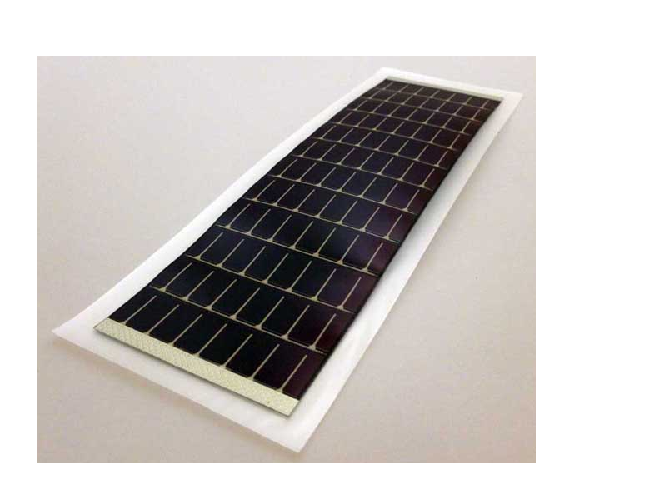
\includegraphics[width=0.7\textwidth]{figures/SolarCell_RC7-2_Powerfilm}
\end{minipage}
\hspace{5mm}
\begin{minipage}[t]{0.55\linewidth}
\centering
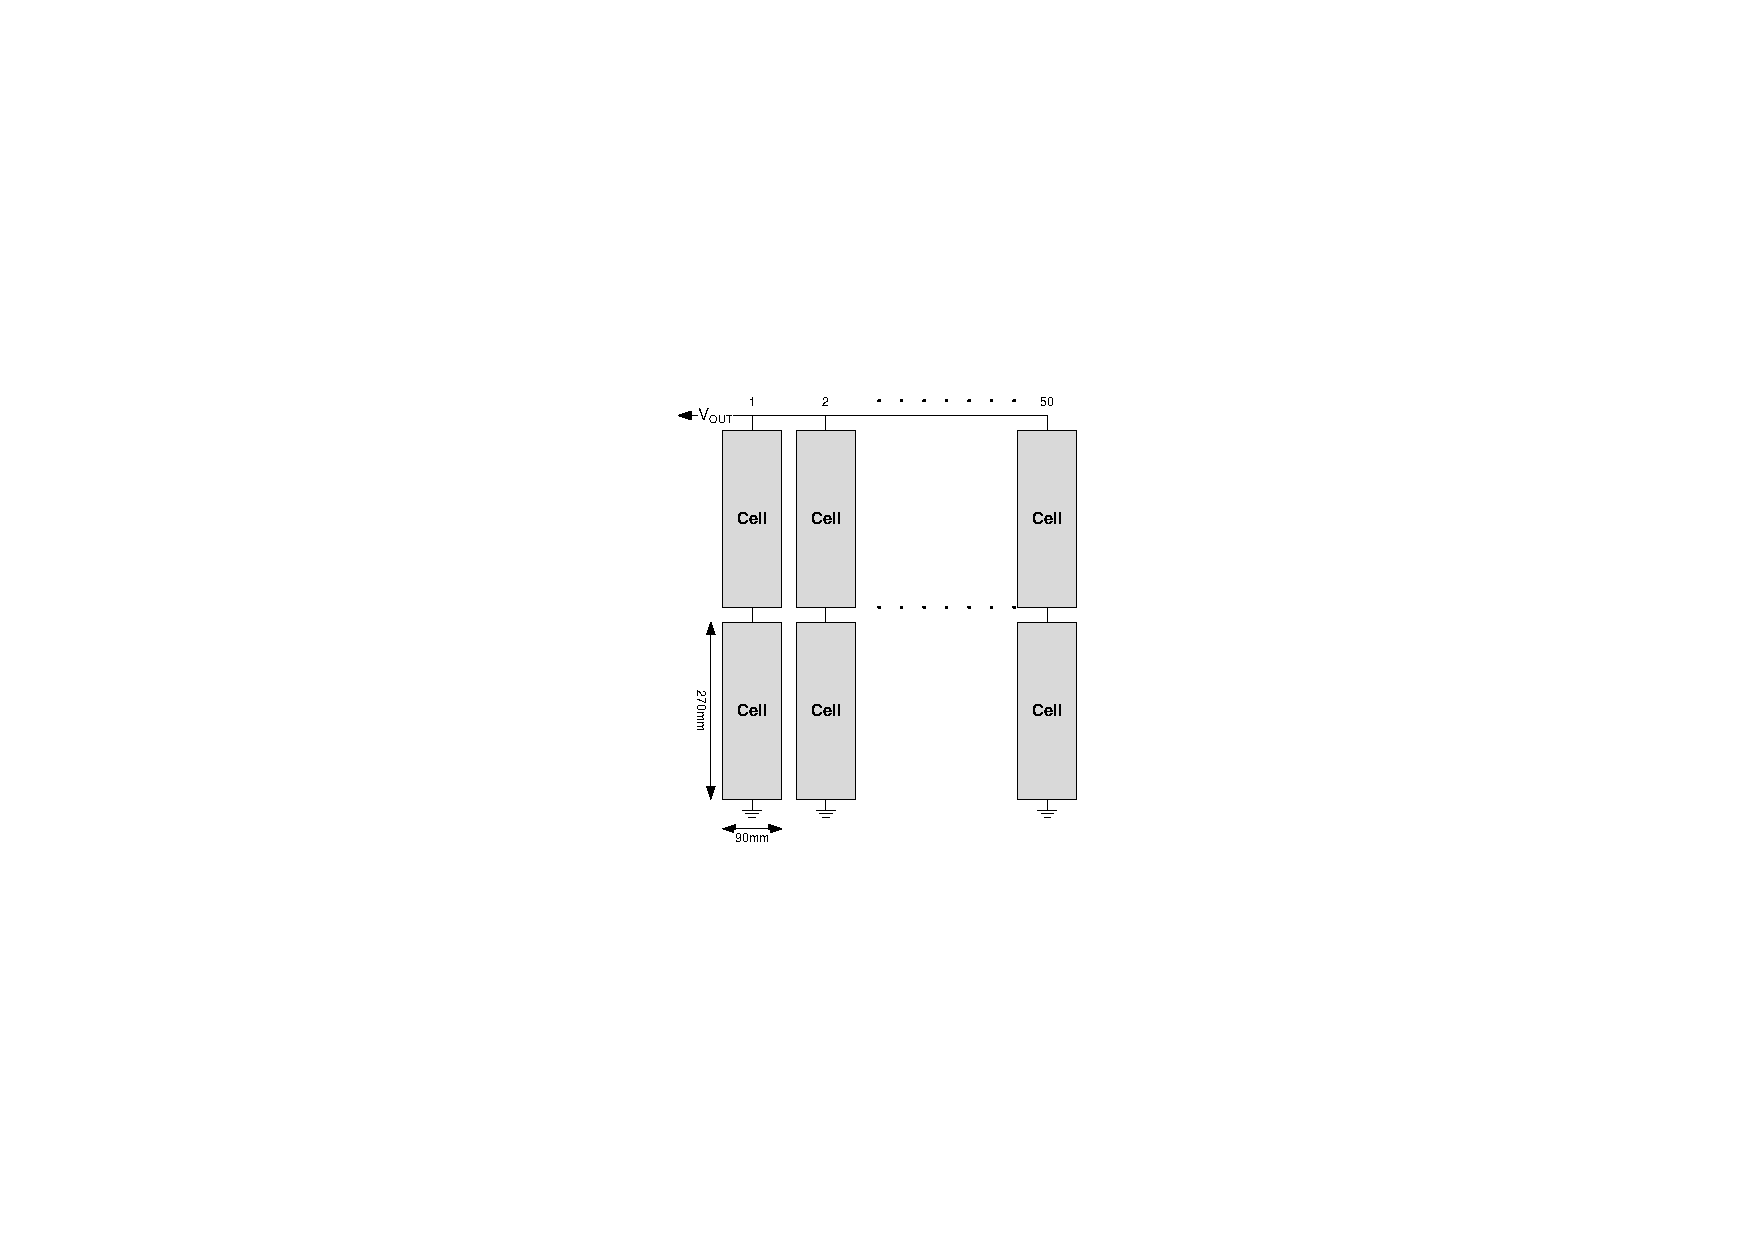
\includegraphics[width=\textwidth]{figures/fig_CDR_Solar_Array}
\end{minipage}
\caption{PowerFilm solar cell(left), Solar array configuration(right)}
\label{fig:solar_cell}
\end{figure}

Since only two cell are in series, it is estimated that bypass diodes are not very beneficial for mitigating shading issues, as was discussed in Section \ref{subsec:environmental_requirements}, and hence are not included in the design.

\subsection{Solar Array Regulator}
The \ac{SAR} must control the optimal the solar array operating voltage as well as limit the output mainbus voltage. A simple step-down buck converter topology is preferred for a number of reasons:

\begin{itemize}
\item simple circuit analysis and low components count
\item no inherent \ac{RHPZ} in contrary to the standard boost topology
\item step-down topology calls for a high input voltage which leads to low input current thus minimizing ohmic losses and the relative forward voltage drop loss from the reverse protection diode
\end{itemize}


\subsubsection{Buck Converter Circuit Design}
The ideal transfer function for the buck converter shown in Figure \ref{fig:EPS_diagram_detailed} is given as

\begin{equation}
V_{out}=D\,V_{in}
\end{equation}

where $D$ is the duty cycle of the MOSFET switch, thus the converter controls the output voltage by varying the duty cycle. This duty cycle is controlled by a \ac{PWM} controller providing input to a high-side MOSFET driver. A \ac{MEA} measures the mainbus output voltage to generate a control signal for the PWM controller. An \textit{LM3477} chip is selected which combines \ac{PWM} controller, \ac{MEA} and gate driver in one single \ac{IC}.\\
The \ac{CM} control scheme is adopted due to its excellent dynamic abilities[REF] and simplified feedback regulator design. A low resistance $10\,m \Omega$ precision sense resistor measures the inductor current slope. The \textit{LM3477} has build-in slope compensation[REF], to avoid current mode instabilities[REF].

The converter switching frequency, $f_{switch}$, is chosen relatively high to $500\,kHz$. The increased switching losses are out-weighted by the fact that the low input voltage limits these losses and high frequency allows the inductor and filter components to be made smaller thus limiting the resistive losses which are expected to dominate converter losses due to the relatively high currents.

The inductor current ripple, $\Delta I_L$, is given by 

\begin{equation}
\Delta I_L=\dfrac{V_{in}-V_{out}}{L\,f_{switch}}D
\end{equation}

where $L$ is the inductance and $f_{switch}$ the converter switching frequency. The inductor current ripple is usually limited to about $10\,\%$ of the maximum output current which was given in Table \ref{tab:technical_requirements} as $10.8\,A$. Thus the minimum required inductance is calculated to

\begin{equation}
L=\dfrac{V_{in}-V_{out}}{\Delta I_L\,f_{switch}}D=\dfrac{14.4\,V-7.4\,V}{1.08\,A 500\,kHz}\cdot 0.514=6.7\,uH
\end{equation}

A $10\,uH$ inductor is chosen giving a current ripple of $0.72\,A$, the converter will enter \ac{DCM} at light loads when the load current drops below $0.36\,A$ which is unlikely to happen in most operating modes.

For the converter output capacitor, a component is chosen which has very low \ac{ESR} and high capacitance to limit the output voltage ripples.

\subsubsection*{Current Sense Amplifier}
With an inductor current ripple of $0.72\,A$ the current sense voltage slope is only 

\begin{equation}
v_{sense}=\Delta I_L\cdot R_{sense}=0.72\,A\cdot 10\,m\Omega = 7.2\,mV
\end{equation}

It is recommended that the slope compensation is equal to or the double of the sense slope[REF], however the minimum compensation slope is limited to $103,mV$ by the LM3477 chip. Thus the sensed slope signal must be amplified with a gain of around 20 being suitable. This also has the advantage of eliminating some of the typical noise susceptibility in the current sense signal. The current sense circuit in Figure \ref{fig:EPS_diagram_detailed} consists of two differential OpAmps which amplifies the current sense slope. Resistive voltage dividers are placed on the OpAmp inputs to scale down the input voltage signals to always be below the $5\,V$ OpAmp supply voltage.

\subsubsection{Maximum Power Point Tracker}
In \cite{PDR} it was decided to use a \ac{MPPTU} with the \ac{SAR} to increase solar array efficiency during changing environment conditions.

The \ac{SAR} with \ac{MPPT} can operate in three different operation regions:
%
\begin{itemize}
\item Battery discharge - when the solar array input power is insufficient to cover the load power demand, the battery is slowly discharged in order to maintain the output voltage. The \ac{MPPTU} controls the input voltage.
\item Battery charge - when the solar array input is greater than the load power, excessive power is used to recharge the battery. The \ac{MPPTU} controls the input voltage.
\item Input power limitation - when the battery is fully charged, the regulator will operate the solar array at a non-optimal voltage, thus limiting the input power to keep the output voltage at a maximum limit. The extra potential input power is dissipated as heat externally on the solar arrays.
\end{itemize}

It is preferred to implement an analog \ac{MPPTU} mainly since this makes the circuit independent on a control signal from a more complicated external \ac{MCU} or \ac{DSP} thus allowing a flexible plug'n-play system to be implemented. 

The \ac{MPPT} has not been completely designed yet.


\subsection{Battery Design}
An Ansmann \ac{LiPo} Racing Pack 2S1P 30C battery is selected. The battery specifications are listed in Table \ref{tab:proposed_battery}

\begin{table}[H]
\centering
\caption{Specification of chosen battery}
\label{tab:proposed_battery}
\begin{tabular}{p{0.4\textwidth}p{0.2\textwidth}p{0.4\textwidth}}
\hline
\textbf{Description} & \textbf{Symbol} & \textbf{Value}\\
\hline 
Chemistry & - & Li-Polymer\\
Nominal voltage & $V_{bat}$ & $7.4\,V$\\
Capacity & $C_{bat}$ & $2.1\,Ah$ / $15.54\,Wh$\\
Weight & $W_{bat}$ & $122\,g$\\
Dimensions & - & $105\,mm\:\times\:35.2\,mm\:\times\:17\,mm$\\
Maximum fast charge current & $I_{charge,max}$ & $3\,A$\\
Maximum discharge current (continuous) & $I_{discharge,max}$ & $63\,A$\\
\hline
\end{tabular}
\end{table}


\subsubsection{Battery Charge Regulator}
%
From the battery datasheet, maximum charge current is $I_{REG}=3\,A$. From the \ac{BCR} datasheet, the minimum current sense resistor value is calculated as
%
\begin{equation}
\begin{split}
R_{sense}=&\dfrac{V_{FCS}}{I_{REG}}\\
R_{sense}=&\dfrac{120\,mV}{3\,mA}=40\,m\Omega
\end{split}
\end{equation}
%
A $50\,m \Omega$ current sense resistor is selected leading to a charge current of $2.4\,A$.
%
The required thermal rating of the pass transistor is calculated as
%
\begin{equation}
P_{max}=(V_{in,max}-V_{bat,min})\cdot I_{charge}=(9.5\,V-5.5\,V)\cdot 2.4\,A=9.6\,W
\end{equation}
%
A TPCA8102 P-channel MOSFET is selected as charge transistor. It has a peak power dissipation rating of $42\,W$ and $1.6\,W$ continuous ($10\,s$) and $R_{DS(ON)}=4.5\,m \Omega$. At $2.4\,A$ charge current, the heat dissipation is well below the maximum allowed value.

\subsubsection*{Voltage Feedback Divider}
To charge the battery, the main bus output voltage must be above the \ac{UVLO} maximum start threshold at $8.9\,V$. $9.5\,V$ is selected, to allow some margin. The \ac{PWM} controller voltage feedback input must be $1.270\,V$ thus determining the feedback voltage divider resistor values to $R_{FB1}=12.9\,k \Omega$ and $R_{FB2}=2\,k \Omega$.
%
%\subsubsection{Battery Temperature Monitoring}
%%
%The \ac{BCR} chip includes a temperature monitoring feature. The battery is rated, in charge-mode, to temperature in the interval $10-45^{\circ}C$. The maximum allowed temperature is set slightly lower to $40^{\circ}C$. The Li-ion battery has a build-in \ac{NTC} thermistor with $B=3980\,K$ and $R_{25}=10k\,\Omega$. The required restance values of the temperature control resistors are determined from the \ac{BCR} chip datasheet as 
%%
%\begin{equation}
%\begin{split}
%R_{cold}&=R_{25}e^{B(\dfrac{1}{T}-\dfrac{1}{T_0}}=10\,k\Omega e^{3980\,K(\dfrac{1}{283	\,K}-\dfrac{1}{298\,K})}=20.3\,k\Omega\\
%R_{hot}&=10\,k\Omega e^{3980\,K(\dfrac{1}{313	\,K}-\dfrac{1}{298\,K})}=5.3\,k\Omega\\
%R_{T1}&=2\dfrac{R_{cold}R_{hot}}{R_{cold}-R_{hot}}=14.2\,k\Omega\\
%R_{T2}&=2\dfrac{R_{cold}R_{hot}}{R_{cold}-3R_{hot}}=47.8\,k\Omega
%\end{split}
%\end{equation}

%
%\subsubsection{Battery Discharge Current Limiter}
%%
%The battery in \cite{panasonic} has a maximum discharge rate current of $I_{discharge}=1.455\,A$. A discharge current limiter circuit has been added as shown in Figure \ref{fig:EPS_diagram_detailed}. In normal conditions, the MOSFET is off making the base pin of the \ac{PNP} \ac{BJT} low and hence the BJT is fully conducting. When the current through the sense resistor increases, the voltage on the PNP MOSFET gate starts to drop and at the current limit point begins to conduct. When this happens, the base of the BJT is pulled up on the device starts to limit the current.
%
%The selected MOSFET has a typical gate threshold voltage of $V_{Gth}=550\,mV$. The chosen \ac{BJT} has a typical collector-emitter voltage drop of $V_{CE}=120\,mV$. The required current sense resistor is then calculated as 
%%
%\begin{equation}
%\begin{split}
%V_{sense}&=V_{Gth}-V_{CE}=550\,mV-120\,mV=430\,mV \Rightarrow\\
%R_{sense}&=\dfrac{V_{sense}}{I_{discharge}}=\dfrac{430\,mV}{1.455\,A}=295\,m\Omega
%\end{split}
%\end{equation}
%%
%The exact required resistance must be determined by testing the precise parameters of the discrete components. The $500\,\Omega$ resistor value is chosen as a compromise between the power loss from current drawn in current limitation mode $P_{loss}\approx V_{bat}^2/R_2$ and the requirement that the resistor must allow about $10\,mA$ (base current) to be drawn at the lowest voltage across the resistor which is about $5\,V$.
%%
%

%\subsubsection{Mainbus Under Voltage Protection}
%%
%The power from battery and solar cells is limited. It is thus possible that the motors will try to draw more current than what can be delivered. If this happens, the output capacitor of the \ac{SAR} will quickly discharge and the main output voltage drops out. To prevent this situation, an \ac{UVP} circuit is added. This is implemented using an $STN888$ PNP \ac{BJT} along with two resistors, $R3$ and $R4$ as shown in Figure \ref{fig:EPS_diagram_detailed}. When the main output voltage is around $6.2\,V$ the Base-Emitter voltage drop is close to $1.2\,V$ and the \ac{BJT} is fully conducting and effectively works as a short circuit. If the output voltage drops significantly below $6.2\,V$ the \ac{BJT} will begin to decrease the output current until the output voltage stabilizes. The current gain of $STN888$ is about $100$, hence to allow an maximum output current of $10\,A$, the resistors $R3$ and $R4$ must be designed to pass $100\,mA$ at $6.2\,V$ output voltage. To minimize efficiency it is important that the forward voltage drop of the \ac{BJT} is kept as low as possible.
%
%\subparagraph*{Further Recommendations}
%%
%It is hard to find suitable \acp{BJT} rated for much more than $5\,A$. If the power output is increased in future designs, it is suggested to either parallel connect several \acp{BJT} however this might cause issues with thermal runaway. Alternatively high current \acp{IGBT} can be used, however they have higher forward voltage drops and thus they are more suitable for a design with a higher output voltage.


%
\subsection{Complete EPS Diagram}
%
The complete \ac{EPS} diagram is shown in Figure \ref{fig:EPS_diagram_detailed}. For providing the $5\,V$ regulated voltage to the payloads, \ac{COTS} DC-DC regulator(s) are used. The battery charging/discharging is controlled by the \ac{SAR}.
%
\begin{sidewaysfigure}
\centering
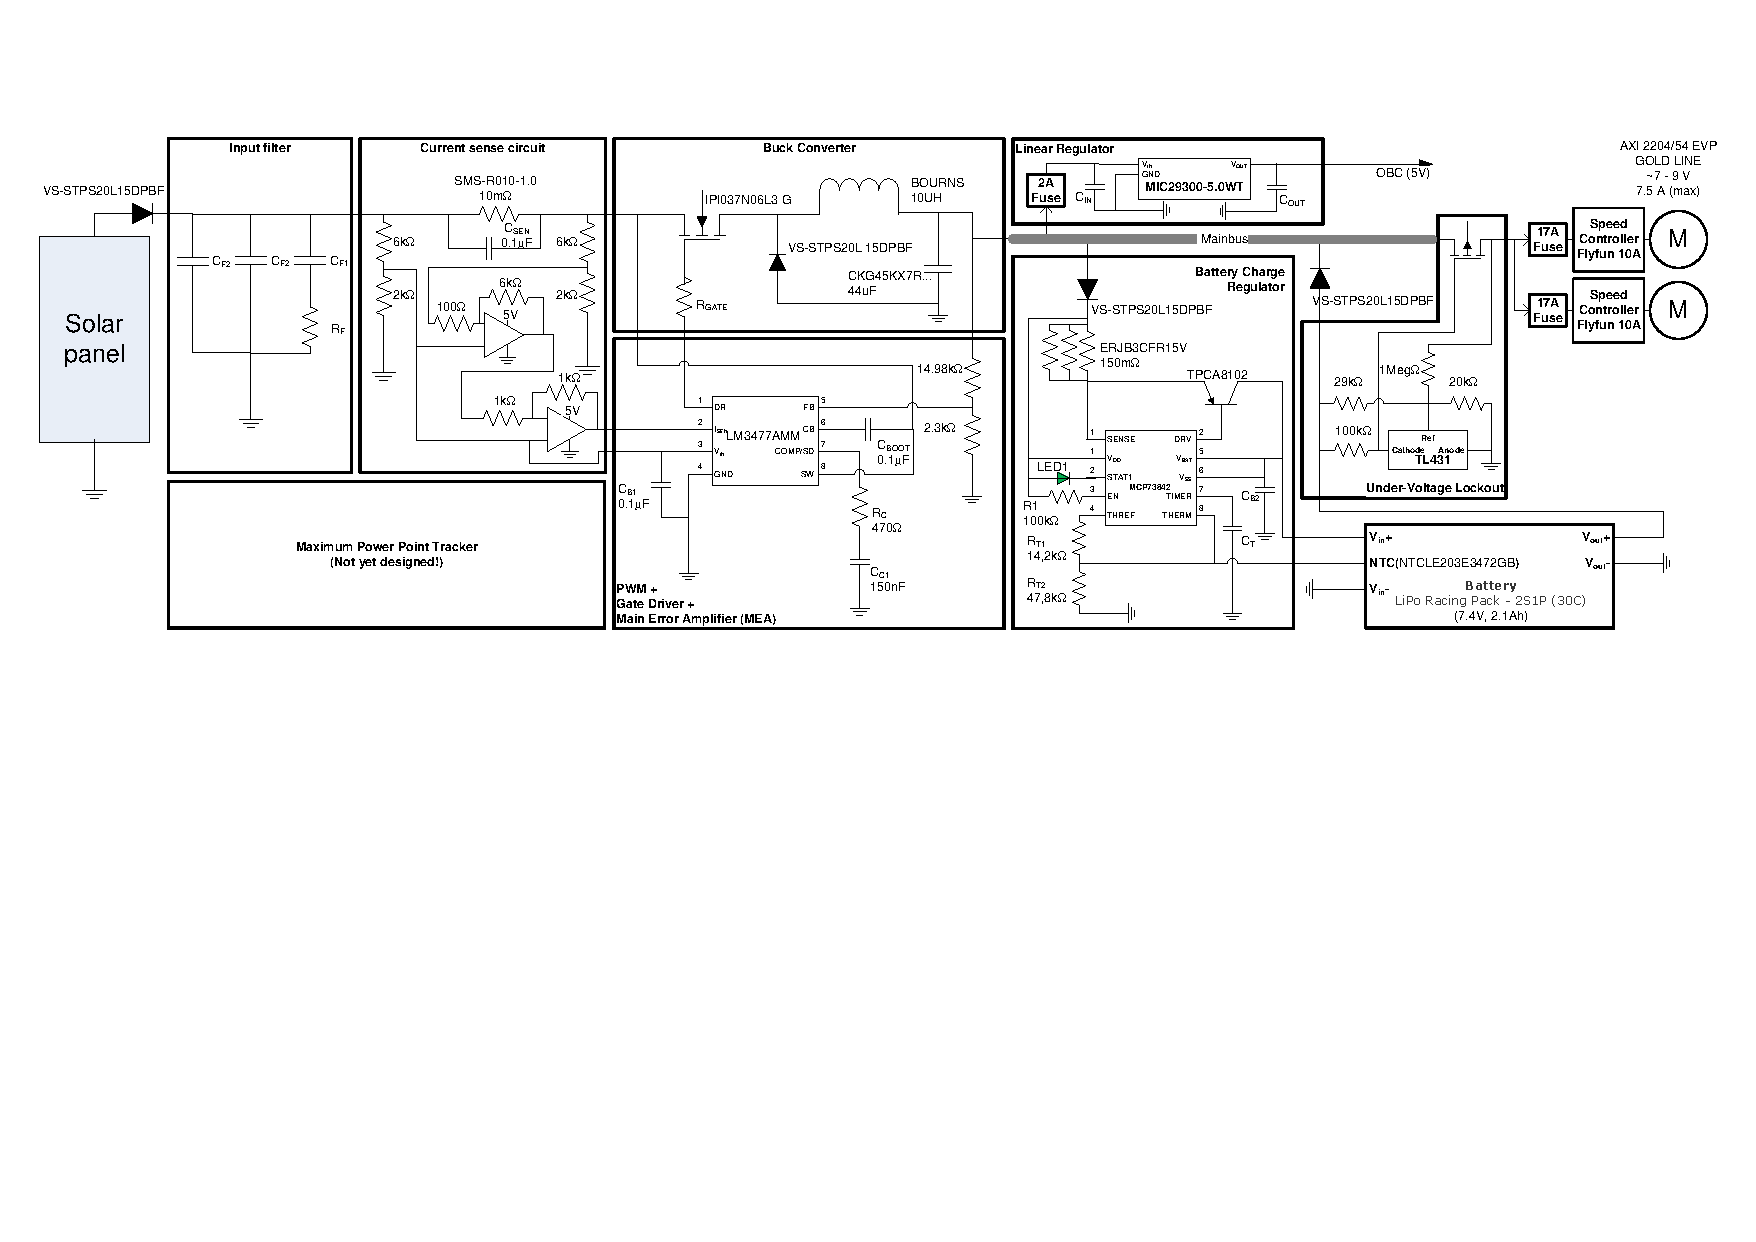
\includegraphics[scale=0.8]{figures/fig_CDR_EPSdiagram_detailed}
\caption{\ac{EPS} detailed block diagram diagram}
\label{fig:EPS_diagram_detailed}
\end{sidewaysfigure}

%
\subsection{External Interfaces}
%
The interfaces of the \ac{EPS} external are listed in table \ref{tab:external_interfaces}.
%
\begin{table}[H]
\centering
\caption{External interfaces}
\label{tab:external_interfaces}
\begin{tabular}{m{0.35\textwidth}m{0.55\textwidth}}
\hline
\textbf{External interface} & \textbf{Implementation}\\
\hline
Solar cells mounting & \ac{PSA}\\[2mm]
DC-DC regulators & Mounted on PCB which sits in system housing. Thermal contact points should be included, to remove internal heat dissipation.\\[2mm]
Battery telemetry & Analog signals to Microcontroller\\[2mm]
Mounting of batteries & \ac{TBD}\\
%Output voltage control(reference voltage setpoint) & Analog signal from Microcontroller\\[2mm]
Supply voltages & $6.0-9.2\,V$ (unregulated) and $5.0\,V$(regulated)\\[2mm]
\hline
\end{tabular}
\end{table}
%
%
\subsection{Telemetry and Telecommands}
%What telemetries/telecommands are required/useful for the subsystem? – What data rates/sizes are required?
%
The required/recommended telemetry and telecommands, \ac{EPS} , are listed in table \ref{tab:Telemetry_Telecommands}.
%
\begin{table}[H]
\centering
\caption{Telemetry and telecommands}
\label{tab:Telemetry_Telecommands}
\begin{tabular}{|l|l|l|}
\hline
\textbf{Telemetry} & \textbf{Data rate/frequency} & \textbf{Data size} \\
\hline
Battery voltage & Every 30 sec & 2 bytes\\
\hline
Battery temperature & Every 5 sec & 2 bytes\\
\hline
%Solar array temperature & Every 30 sec & 1 byte\\
%\hline
%Solar array voltage & Every 1 sec(MPPT performance) & 2 bytes\\
%\hline
%Solar array current & Every 1 sec(MPPT performance) & 2 bytes\\
%\hline
\end{tabular}
\end{table}